\documentclass{article}

\usepackage[english]{babel}

\usepackage[letterpaper,top=2cm,bottom=2cm,left=3cm,right=3cm,marginparwidth=1.75cm]{geometry}
\usepackage{amsmath}
\usepackage{graphicx}
\usepackage[colorlinks=true, allcolors=blue]{hyperref}



\title{Transfer Learning for Cypher Difficulty Classification with Noisy Large‑Scale Labels and Curated Fine‑Tuning}
\author{Nada Bou Kanaan \\ Algorithms for massive datasets Project\\ Master in Computer Science}

\begin{document}
\maketitle


\section{Goal}

Implement a model that classifies Cypher queries by difficulty level (node level, 1 hop, 2 hop, 3 hop, hard level), trained on a large dataset and adaptable to new data. (Definitions of Cypher queries and difficulty levels are given in the appendix.)


\section{Problem}

In the literature, large text to cypher datasets are often generated and labeled by LLMs, which makes label quality potentially unreliable.
A notable example is the Neo4j text2cypher dataset with  about 44,000 entries and a highly imbalanced difficulty distribution.
More generally, in LLM generated datasets, queries labeled as hard often do not satisfy all difficulty criteria. As a result, a model trained only on this type of data may struggle with hard queries defined using different criteria

Manually curated datasets (both generation and labeling) are much rarer and usually small because they are costly to produce. I created a smaller but high-quality dataset consisting of 2,500 queries, balanced across difficulty levels (500 per level).


Figure 1 illustrates the imbalance in the Text2Cypher dataset

\begin{figure}
\centering
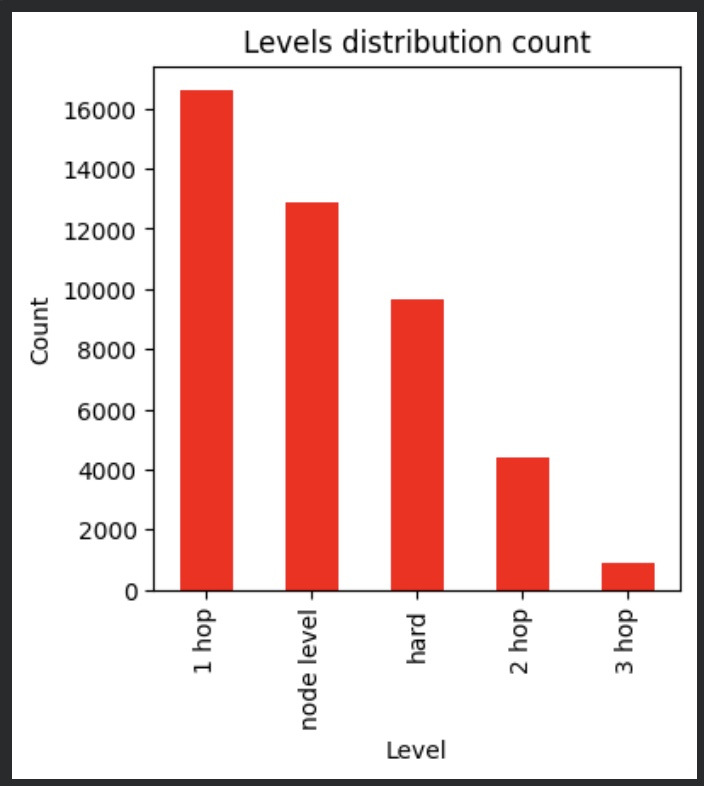
\includegraphics[width=0.25\linewidth]{Immagine.jpg}
\caption{\label{fig:composition}  Text2Cypher difficulty level distribution.}
\end{figure}


\section{Datasets considered}
\begin{enumerate}
\item Text2Cypher (Neo4j, about 44,000 entries)
The Neo4j Text2Cypher dataset was released on November 7, 2024 and accessed from the Hugging Face repository (in March 2026). I downloaded it and manually re-labeled it for the purposes of this project.\footnote{\url{https://neo4j.com/blog/developer/introducing-neo4j-text2cypher-dataset/}}

Strengths: large size.

Weaknesses: highly imbalanced: some levels are extremely rare, the hard level queries do not cover all difficulty criteria.

\item Curated dataset (2,500 entries).
Dataset created entirely by me.

Strengths: balanced, high quality, manually labeled, complete coverage of hard-level criteria.

Weaknesses: small size.

\end{enumerate}

\textbf{Data access} The datasets are downloaded at runtime from private Google Drive links using \texttt{gdown}. 



\section{Proposed approach}

To achieve my goal, I labeled the Neo4j Text2Cypher dataset (manually curated labeling) to make it suitable for training,  and I conducted a series of experiments by implementing different methodologies to identify the most efficient one

\begin{enumerate}
\item Approach 1

Use a pretrained model (CodeBERT), train it on Text2Cypher, evaluate on its test set, then evaluate on the curated dataset.

CodeBERT is a pretrained model for programming languages, trained on large-scale code corpora (NL--PL pairs).\footnote{\url{https://aclanthology.org/2020.findings-emnlp.139/}}


\item Approach 2
Train CodeBERT on the concatenated dataset (Text2Cypher + curated), evaluate as above.

\item Approach 3
Train CodeBERT on Text2Cypher, then fine-tune on the curated dataset, evaluate as above.

\item Approach 4
Implement a from scratch neural network baseline and train it on the concatenated dataset, to compare against the pretrained model.

\end{enumerate}

\section{Implementation and Results}



\subsection{Pretrained trained on Text2Cypher }

I fine-tuned CodeBERT on the large Text2Cypher dataset, with an optional subsampling  step (training is performed in mini‑batches on GPU) to control runtime, and it can scale to the full dataset when subsampling is disabled (I used 50\% of the data). For this purpose, I first loaded the required libraries and datasets, and normalized the labels to ensure consistency across the different data sources. Then I defined the main training configuration, including the hyperparameters, and applied stratified subsampling because the dataset is highly imbalanced. This was done to preserve class proportions and reduce the risk of excluding rare classes during sampling. The train, validation, and test splits were also created using stratification in order to maintain the same class distribution across all subsets.

The model was trained using a standard PyTorch training loop with cross-entropy loss and the predefined hyperparameters. At each epoch, the model was set to training mode, batches were moved to the GPU, a forward pass was performed, the loss was computed, gradients were backpropagated, and the optimizer updated the model weights. Predictions were collected throughout training in order to compute accuracy and macro-F1, which is appropriate here because the task involves five classes. A separate evaluation loop was run on the validation set in evaluation mode and without gradient computation to assess generalization performance. Training and validation losses were recorded and plotted over time.

Finally, the trained model was saved and evaluated both on the Text2Cypher test set and on the curated dataset, with particular attention to its hard-level subset, in order to assess performance under different labeling criteria.
 

\textbf{Results}

\textit{On Text2Cypher:}
\[
\text{Accuracy} = 0.9988 \qquad \text{F1} = 0.9985
\]

\textit{On the curated dataset (hard level only):}
\[
\text{Precision} = 0.9867
\]
\[
\text{Recall} = 0.7420
\]
\[
\text{F1} = 0.8470
\]



\subsection{Pretrained trained on concatenated}

In this experiment, I merged the Text2Cypher dataset with my curated dataset into a single training set and fine-tuned CodeBERT once on the combined data. The same preprocessing steps, label normalization, and training pipeline were applied. The goal was to introduce higher-quality labels directly into the large-scale training phase and evaluate whether this single-stage training on merged data could improve performance, especially with respect to the hard-level criteria.
\textbf{Results}

\textit{On Text2Cypher:}
\[
\text{Accuracy} = 0.9968 \qquad \text{F1} = 0.9906
\]

\textit{On the curated dataset (hard level only):}
\[
\text{Precision} = 0.9827
\]
\[
\text{Recall} = 0.9080
\]
\[
\text{F1} = 0.9439
\]

\subsection{Pretrained trained on Text2Cypher + fine-tuning }

The model is first fine‑tuned on the large Text2Cypher dataset.
The resulting model was then fine-tuned a second time on the curated dataset using a smaller learning rate and fewer epochs. This two-stage strategy was designed to adapt the model to the more generic hard-level criteria while preserving the broader knowledge learned from the large dataset, and keeps the pipeline flexible so it can be updated as new curated data becomes available. Evaluation was carried out on both the Text2Cypher test set and the curated dataset in order to assess the trade-off between generalization and alignment with the curated labels.

\textbf{Results}

\textit{After the first training stage:}

\textit{On Text2Cypher:}
\[
\text{Accuracy} = 1.0000 \qquad \text{F1} = 1.0000
\]

\textit{On the curated dataset (hard level only):}
\[
\text{Precision} = 0.9868
\]
\[
\text{Recall} = 0.7460
\]
\[
\text{F1} = 0.8497
\]

\textit{After the second training stage:}

\textit{On the curated dataset (hard level only):}
\[
\text{Precision} = 0.9568
\]
\[
\text{Recall} = 0.9300
\]
\[
\text{F1} = 0.9432
\]

\subsection{ Neural Network baseline from scratch}

I implemented a fully supervised model without pretrained weights (using the combined dataset). Each Cypher query was converted into a TF-IDF vector, that is, a bag of words representation in which tokens and short token sequences are weighted according to their importance. I used \(n\)-grams (unigrams and bigrams) so that the model could capture both individual keywords and short phrases, while TF-IDF weighting emphasized terms that are frequent in a specific query but rare across the corpus. These vectors were then used as input to a small MLP with two hidden layers, ReLU activations, and dropout. The network was trained using cross-entropy loss and evaluated on the same train/validation/test split adopted in the transfer learning experiments.

\textbf{Results}

\textit{On combined:}
\[
\text{Accuracy} = 0.9727 \qquad \text{F1} = 0.9529
\]

\textit{On the curated dataset (hard level only):}
\[
\text{Accuracy} = 0.972
\]
\[
\text{Precision} = 1.0000
\]
\[
\text{Recall} = 0.9720
\]
\[
\text{F1} = 0.9858
\]


\section{Discussion}


The experiments show the effect of label quality and class balance on performance. Models trained only on the large \textit{Text2Cypher} dataset achieve high accuracy on its test set but generalize less well to the curated dataset, especially for the \textit{HardLevel} class, confirming a label-quality shift.

The two-stage fine-tuning improves recall on \textit{HardLevel}, indicating that the curated data helps align the model with wider difficulty criteria. Training on the concatenated dataset yields slightly higher precision on \textit{HardLevel}, while two-stage fine-tuning yields higher recall. The overall F1 score is similar, so the choice depends on whether missing hard queries or producing false hard predictions is more costly. In this case, avoiding missed hard queries is preferable, \textbf{making the two-stage fine-tuning approach the most suitable}, and therefore the pipeline is designed to be updatable so that, as new curated data becomes available, the model can be retrained or fine‑tuned to incorporate it.

The from-scratch TF-IDF + MLP baseline performs surprisingly well, suggesting that the task is partly driven by surface-level patterns. However, the pretrained \textit{CodeBERT} model provides better adaptability under broader labeling definitions.


\section{Appendix — Definitions}

\textbf{Cypher} is Neo4j’s declarative query language for property graphs. A Cypher query specifies graph patterns (nodes and relationships) to match, and applies filters, projections, and aggregations to return results. Its syntax is designed to be readable and to resemble graph structures (pattern matching).\footnote{\url{https://neo4j.com/docs/getting-started/cypher-intro/}}

\textbf{Difficulty levels.} The difficulty is defined by the structural complexity of the Cypher pattern:
\begin{itemize}
\item \textbf{nodeLevel}: single-node patterns, simple return, no relationship traversal.
\item \textbf{1 hop}: one relationship traversal (one edge) in the pattern.
\item \textbf{2 hop}: two consecutive relationship traversals (two edges).
\item \textbf{3 hop}: three consecutive relationship traversals (three edges).
\item \textbf{hardLevel}: A question--Cypher pair is labeled \textbf{Hard} if answering it requires advanced Cypher constructs beyond hop-length traversal, specifically involving non-trivial intermediate bindings, aggregation, hierarchical path expressions, or string/sequence computation. Concretely, a query is Hard if it uses at least one of the following operator families: \emph{List reasoning + conditional logic}, \emph{Multi-stage query pipelines and aggregation with WITH}, \emph{Hierarchical and variable-length path reasoning}, or \emph{Complex compositional filtering}.
\end{itemize}

\section{Declaration}

I declare that this material, which I now submit for assessment, is entirely my own work and has not been taken from the work of others, save to the extent that such work has been cited and acknowledged within the text of my work. I understand that plagiarism, collusion, and copying are grave and serious offences in the university and accept the penalties that would be imposed should I engage in plagiarism, collusion or copying. This assignment, or any part of it, has not been previously submitted by me or any other person for assessment on this or any other course of study. No generative AI tool has been used to write the code or the report content.

\end{document}
